\chapter{Example Output of a Single Segmentation Round\label{app:segmentedOutput}}

This appendix is provided as example to assist in visualizing the different outputs generated during segmentation.  Figure~\ref{fig:segmentationGroundTruthImages} shows the two ground-truth images that were provided to the Mixed-Bag Solver for this example.  As explained in Section~\ref{sec:Segmentation}, the Mixed-Bag solver assembles the pieces from these images as if they had come from a single puzzle; the assembler output for the first round of segmentation is shown in Figure~\ref{fig:segmentationAssemblerOutput}.

The segments present in the assembler output are shown in Figure~\ref{fig:segmentationRepresentation}, with the segments colored to make then easier to identify.  For a given segment, the pieces that are further away from an open location are lighter in color while those closer to a boundary are darker.  The stitching pieces that would have resulted from each segment (assuming it exceeded the minimum segment size) are marked with white crosses.

Figure~\ref{fig:bestBuddiesAssemblerOutput} is the best buddy visualization of the assembler output.  Note that the right and left sides of image (a) have stripes of best buddies that extend only in the horizontal direction.  As such, each piece in those stripes represent articulation pieces.  As such, they were trimmed from the main segment in the center of the image as described in Section~\ref{sec:articulationPoints}.

\begin{figure}
\centering
  \begin{tabular}{ >{\centering\arraybackslash}m{0.47\textwidth} >{\centering\arraybackslash}m{0.47\textwidth} }

	\fbox{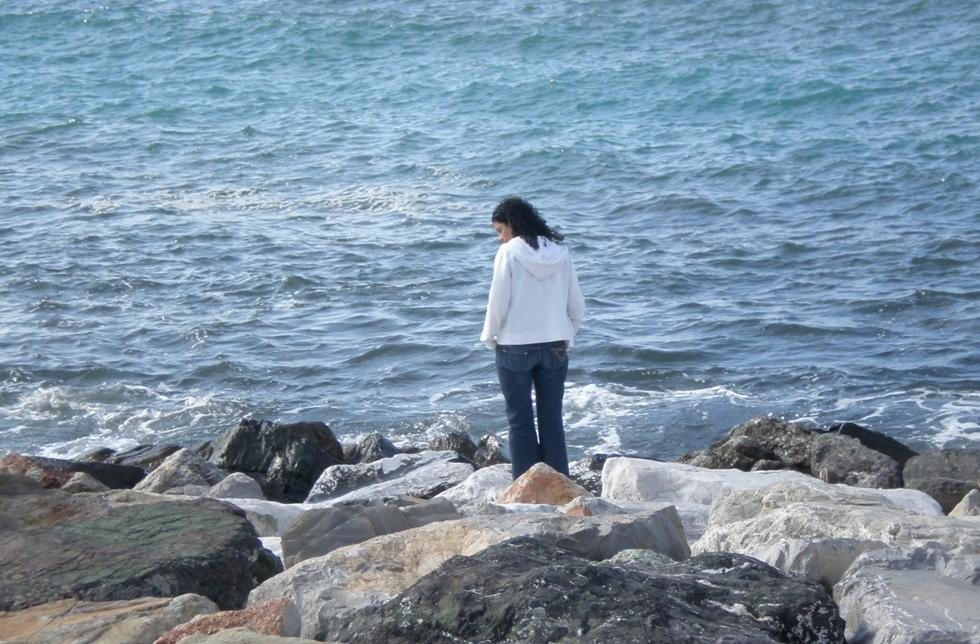
\includegraphics[scale=0.18]{./images/segmentation/pomeranz_805_8.jpg}} & \fbox{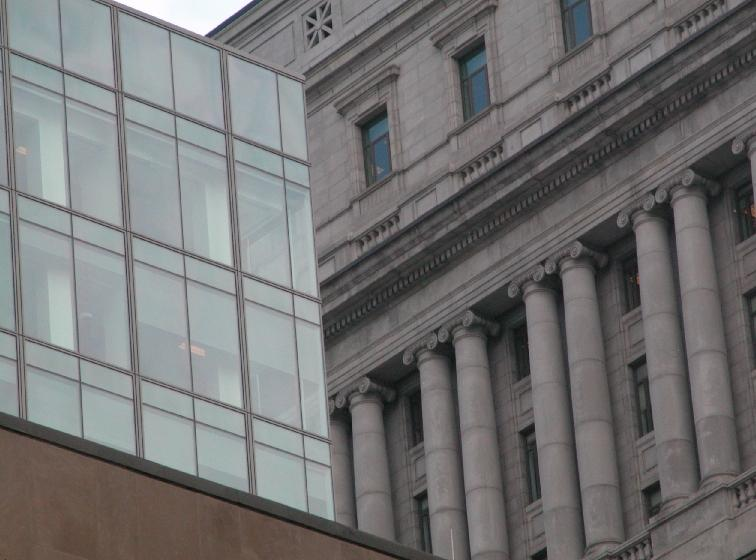
\includegraphics[scale=0.18]{./images/segmentation/mcgill_540_20.jpg}} \\~\\
	Image (a) -- 805 Pieces \ & Image (b) -- 540 Pieces\\~\\
  \end{tabular}

\caption{Segmentation Example Ground-Truth Images}
\label{fig:segmentationGroundTruthImages}
\end{figure}

\begin{figure}
\centering
  \begin{tabular}{ >{\centering\arraybackslash}m{0.47\textwidth} }
	\fbox{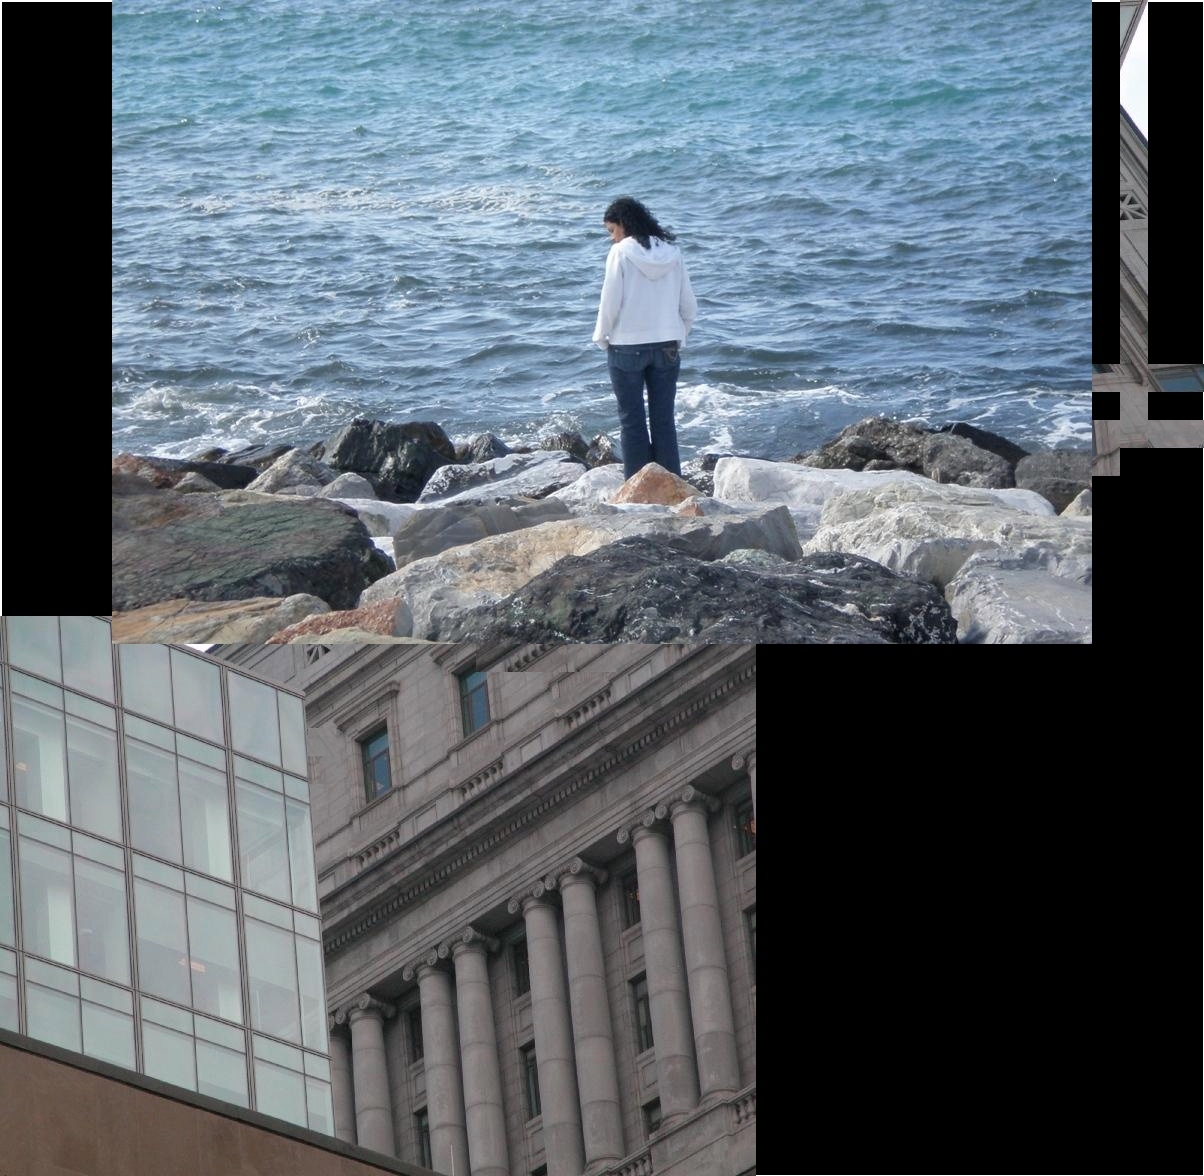
\includegraphics[scale=0.18]{./images/segmentation/assembler_single_puzzle_output.jpg}} \\~\\
  \end{tabular}

\caption{Example Assembler Output of a Single Puzzle after the First Segmentation Round}
\label{fig:segmentationAssemblerOutput}
\end{figure}

\begin{figure}
\centering
  \begin{tabular}{ >{\centering\arraybackslash}m{\textwidth} }
	\fbox{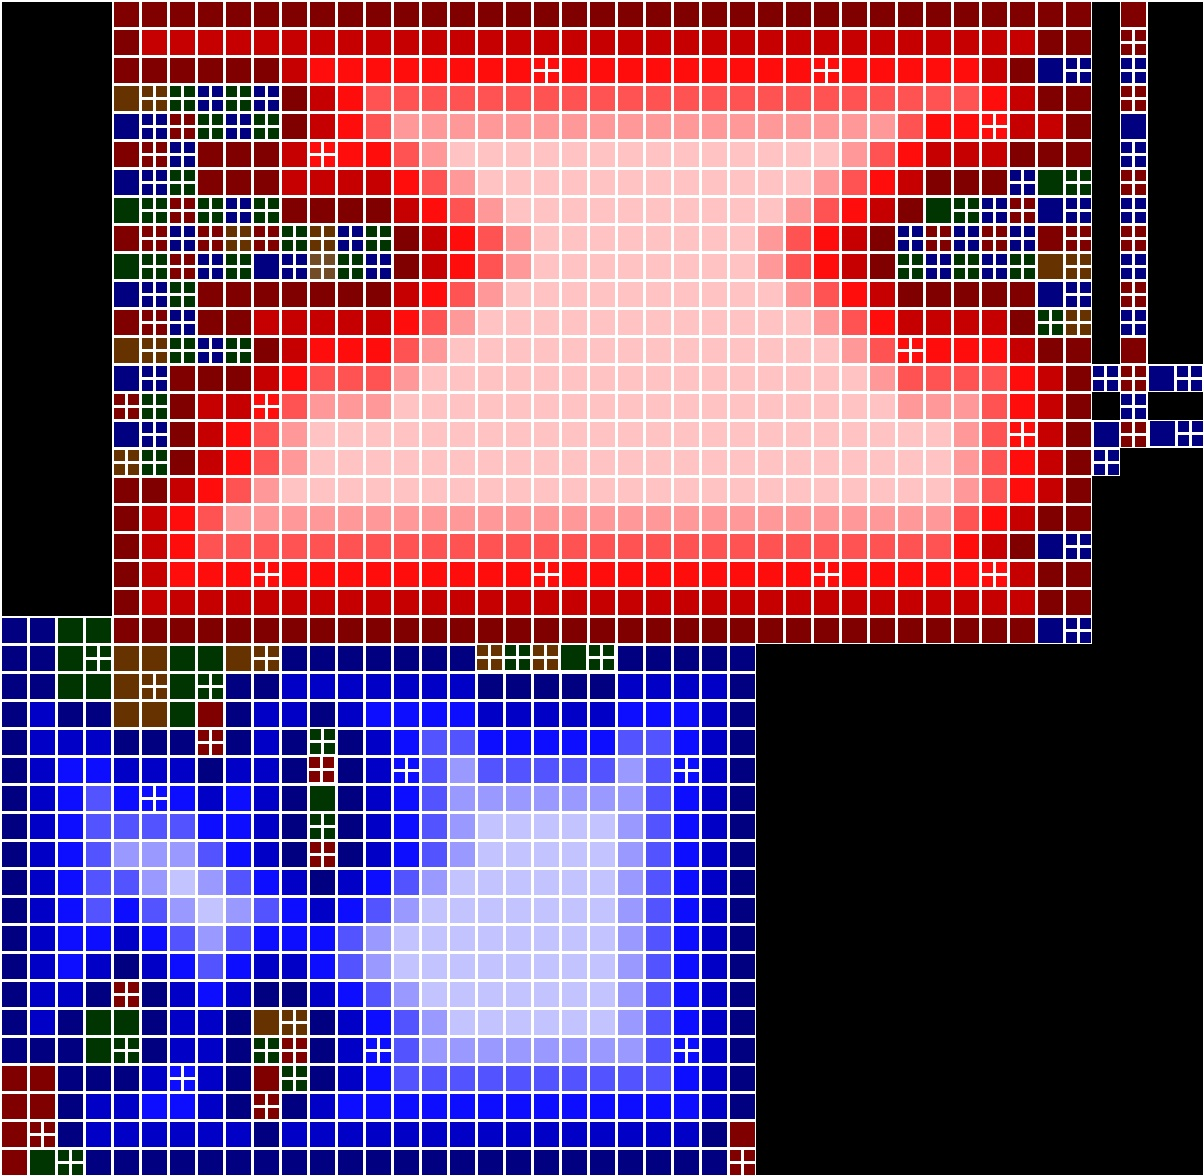
\includegraphics[scale=0.18]{./images/segmentation/segmentation_assembler_output.jpg}} \\~\\
  \end{tabular}
\caption{Segmentation of the Assembler Output}
\label{fig:segmentationRepresentation}
\end{figure}

\begin{figure}
\centering
  \begin{tabular}{ >{\centering\arraybackslash}m{\textwidth} }
	\fbox{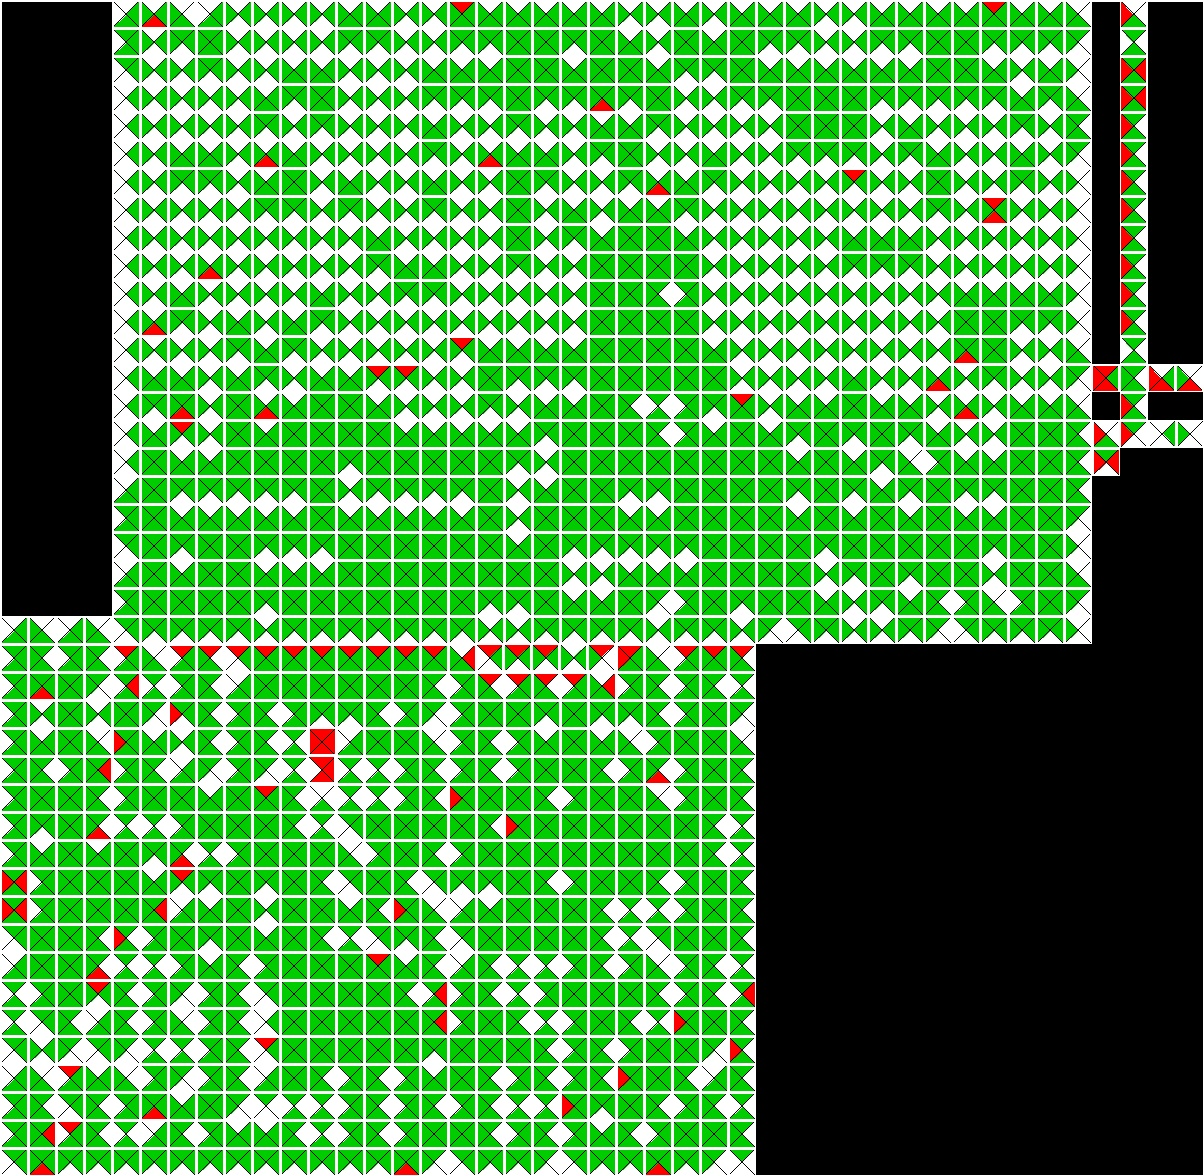
\includegraphics[scale=0.18]{./images/segmentation/best_buddy_assembler_output.jpg}} \\~\\
  \end{tabular}
\caption{Best Buddy Visualization of the Assembler Output}
\label{fig:bestBuddiesAssemblerOutput}
\end{figure}
